\documentclass[11pt]{article}

\usepackage[T1]{fontenc}
\usepackage[polish]{babel}
\usepackage[utf8]{inputenc}
\usepackage{lmodern}
\usepackage{multirow}
\selectlanguage{polish}
\usepackage{graphicx}
\usepackage{listings}

\begin{document}
Java jest wysokopoziomowym, kompilowanym, obiektowym językiem programowania z silną kontrolą typów. Oznacza to, że każda zmienna musi zostać zadeklarowana przed użyciem. 

\section{Typy danych}
Zmienne w javie dzielą się na trzy rodzaje typów
\subsection{typy proste - prymitywy}
Typy prymitywne służa do reprezentacji danych, nie będących obiektami\footnote{istnieją również typy obiektowe reprezentujące typy proste}. Są one wbudowane w język. Ważną cechą jest, że ich wielkość (rozmiar) nie zależy od konkretenej implementacji maszyny wirtualnej. Wyróżniamy osiem typów prostych, które można dodatkowo pogrupować ze względu na \textit{charakter}: typy całkowiete, zmiennoprzecinkowe, znakowe oraz logiczne.

\begin{table}[h]
\centering
\begin{tabular}{|c|c|c|} 
\hline \textbf{typ wbudowany} & \textbf{rozmiar w bitach} & \textbf{zakres} \\
\hline \multicolumn{3}{|c|}{typy logiczne} \\
\hline boolean & 8 & true / false \\
\hline \multicolumn{3}{|c|}{typy całkowite} \\
\hline byte & 8 & $-128$ do $127$ \\ 
\hline short & 16 & $-2^{15}$ do $2^{15}-1$ \\
\hline int & 32 & $-2^{31}$ do $2^{31}-1$ \\
\hline long & 64 & $-2^{63}$ do $2^{62}-1$ \\
\hline \multicolumn{3}{|c|}{typy znakowe} \\
\hline char & 16 & $0$ do $2^{16}-1$ \\
\hline \multicolumn{3}{|c|}{typy zmiennoprzecinkowe} \\
\hline float & 32 & $1.4e^{-45}$ do $3.4028235e^{38}$ \\
\hline double & 64 & $4.9e^{-324}$ do $1.797e^{308} $ \\

\hline
\end{tabular}
\end{table}

\subsection{Konwersja typów numerycznych}
W przypadku konwersji typów należy rozpatrzeć dwa przypadki - niejawne - nie wymagające użycia operatora rzutowania oraz wymagające jawnego rzutownania.
Rzutowanie automatyczne zachodzi w przypadku przypisywania typu od mniejszej ,,dokładności'' do typu o większej (na diagramie są możliwe operacje, które obrazują czarne strzałki). 
\begin{figure}
\centering
%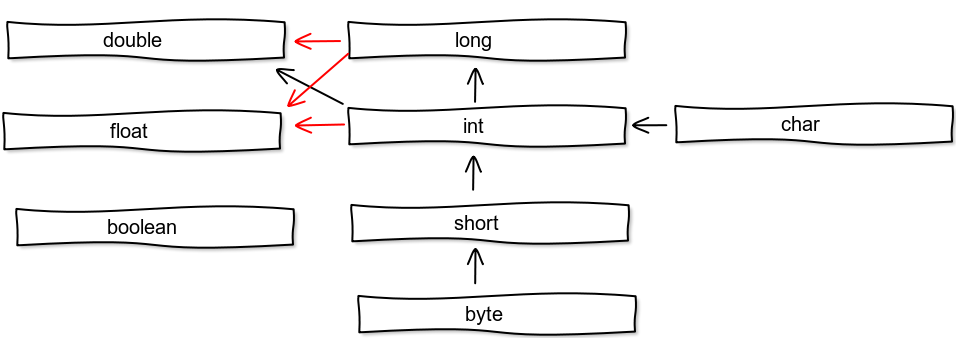
\includegraphics[scale=0.4]{drawing.png}	
\caption{Hierarchia typów}
\end{figure}
Przykładowe konwersje, które nie wymagają jawnego rzutowania, oraz nie powodują utraty danych.
\lstinputlisting{src/widening.java}
Możliwe jest też niejawne rzutowania, które powoduje utradę danych
\lstinputlisting{src/widening-loose.java}
W przykładzie powyżej kompilator nie zgłosi żadnego błędu.\\

W przypadku ,,poruszanie się'' po hierarchii typów w kierunku niezgodnym z kierunkiem strzałek, wymagane jest jawne rzutowanie. Konwesja ta wiąże się z ryzykiem utraty informacji. Przykłady:  
\lstinputlisting{src/casting.java}
Aby wykonać rzutowanie, należy przez nazwą rzutowanej zmiennej postawić nazwę typu docelowego w okrągłych nawiasach.
\subsection{typy obiektowe}
\subsection{typy tablicowe} 
Tablica jest rodzajem struktury danych będąca zestawieniem elementów tego samego typu. Dostęp do każdego z tych elementów można uzyskać za pomocą indeksu w postaci liczby typu int. Przykładowo, jeżeli $\textit{a}$ jest tablicą liczb całkowitych, to $\textit{a[i]}$ jest $\textit{i-tym}$ elementem tej tablicy.\\
Deklaracja zmiennej tablicowej polega na określeniu typu tablicy (czyli podaniu typu elementów i nawiasów kwartatowych $\textit{[]}$) i nazwy zmiennej
\begin{lstlisting}
int [] a;
\end{lstlisting}
Powyższa instrukcja tylko deklaruje zmienną $\textit{a}$. Nie inicjuje jej jednak tablicą (użycie tablicy, przypisanie lub pobranie jakiejś wartości, spowoduje błąd). Do utworzenia tablicy potrzebny jest operator $\textit{new}$
\begin{lstlisting}
int [] a = new int[100];
\end{lstlisting}
Powyższa instrukcja tworzy tablicę, w której można zapisać 100 elementów typy $\textit{int}$.\\
Tablice indeksowane są od zera. Oznacza to, że pierwszy element w tablicy znajduje się pod indeksem 0, natomiast ostatni po indeksem równym $\textit{długości tablicy - 1}$

\section{Przepływ sterowania}
\subsection{Instrukcje warunkowe}
Instrukcje warunkowe służą do podejmowania decyzji, czy dany kod ma być wykonany. Najprostszy warunek ma postać 
\begin{lstlisting}
if (warunek_logiczny) 
	instrukcja
\end{lstlisting}
Warunek zawsze musi zwracać (być ewaluowany do) wartości logicznej true / false. 
\lstinputlisting{src/if.java}
Po $\textit{if}$ mogą, opcjonalnie, wystąpić bloki wykonujące kod w przypadku gdy nie zostanie spełniony właściwy warunek.
\begin{lstlisting}
if (warunek_logiczny) 
	instrukcja1
else
	instrukcja2
\end{lstlisting}
oraz 
\begin{lstlisting}
if (warunek_logiczny) 
	instrukcja1
else if (warunek_logiczny) 
	instrukcja2
else
	instrukcja3
\end{lstlisting}
Bloki $\textit{if()\{ \}}$, $\textit{if() \{ \} else \{ \}}$, $\textit{if() \{ \} else if() \{ \} else \{ \}}$ można dowolnie zagnieżdżać. Przykład
\lstinputlisting{src/if-example.java}
\subsection{Pętle}
Pętla $\textit{while}$ wynonuje blok instrukcji do póki zadany warunek ma wartość $\textit{true}$. Ogólna postać to
\lstinputlisting{src/while.java} 
Jeżeli $\textit{warunek\_logiczny}$ będzie fałszywy przed rozpoczęciem wykonywania bloku $\textit{while}$, instrukcje wewnątrz bloku nie zostaną wykonane. Pętla $\textit{while}$ sprawdza warunek na samym początku działania. W związku z tym jej instrukcje mogą nie zostać wykonane ani razu. Aby mieć pewność, że instrukcje zostaną wkonane co najmniej raz, sprawdzanie warunku trzeba przenieść na sam koniec. Do tego służy pętla $\textit{do-while}$. Jej składnia jest następująca
\begin{lstlisting}
do { 
	instrukcje
} while( warunek_logiczny )
\end{lstlisting}
Najpierw wykonywany jest blok instrukcji, a następnie sprawdzany jest warunek.\\
Ostatnią przedstawioną będzie instrukcja wyboru $\textit{switch}$ (jest ona generalizacją instrukcji if). Składania jest następująca
\begin{lstlisting}
switch (warunek_wyboru) {

	case wartosc1:
		instrukcja1
	case wartosc2:
		instrukcja2
	default:
		instrukcja3

}
\end{lstlisting}
W instrukcji $\textit{switch}$ $\textit{warunek\_wyboru}$ nie jest wyrażeniem logiczny, które ewaluuje do wartości logicznej (true / false). $\textit{Warunek\_wyboru}$ powinien być liczą całkowitą (lub char)\footnote{lub enum}. Natępnie instrukcje z $\textit{case}$, który spełnia warunek, są wykonywane kaskadowo w dół.
\lstinputlisting{src/switch.java}
W powyższym przykładzie, jeżeli wartość wejściowa będzie równa 0, zostanie wyświetlone '0'. W kolejnej linijce znajduje się instrukcja $\textit{break}$, która przerywa działanie $\textit{switch}$.
Jeżeli, wartość wejściowa będzie równa 1, zostaną wyświetlone następujące napisy: '1', '2,3'. '4' nie zostanie wyświetlone ponieważ, poprzedni blok konczy się instrukcją $break$. Jeżeli wartość wejściowa będzie równa, np. 1000, nie zostanie dopawowany żaden warunek i wykona się instrukcja z $\textit{default}$

\section{Klasy}
Program napisany w javie składa się z obiektów. Każdy z nich posiada określony stan, zachowanie, tożsamość. Stan określony przez zmienne, zachowanie definiujemy w metodach, które mogą zmieniać aktualny stan obiektu. Tożsamość pozwala odróżnić dwa obiekty, posiadające ten sam stan, od siebie. \\
Aby utworzyć obiekt, potrzebujemy szablonu, który definiuje dostępne zachowania albo pola, które będą przechowywały stan.\\
  
\subsection{Tworzenie klas}
Klasy przechowywane są w plikach tekstowych (zwyczajowo z rozszerzeniem 'java'). Zdefiniowanych jest szereg reguł dotyczących stworzenia klasy oraz ich struktury
\begin{itemize}
\item w pliku źródłowym może być zdefiniowana tylko jedna klasa $\textit{publiczna}$. Może nie być żadnej.
\item komentarze mogą znajdować się w dowolnym miejscu w pliku
\item nazwa pliku musi być identyczna do nazwy klasy $\textit{publicznej}$. Przykładowo klasa $public class Point { }$ musi znajdować się w pliku o nazwie $Point.java$
\item jeśli klasa umieszczona jest w pakiecie, deklaracja pakietu musi znajdować się w pierwszej linijce (nie uwzględniając komentarzy)
\item definicje importów muszą znajdować się pomiędzy deklaracją pakietu (lub początkiem pliku) oraz definicją pierwszej klasy
\item definicja pakietu oraz importów odnoszą się do całego pliku
\item w pliku źródłowym mogą znajdować się definicje $\textit{nie-publicznych}$ klas
\end{itemize}

Najprostsza definicja klasy składa się z słowa kluczowego $\textit{class}$ oraz nazwy klasy.
\begin{lstlisting}
class Point { }
\end{lstlisting}
Klasa $\textit{Point}$ zdefiniowana w powyższy sposób posiada dodatkowo niejawny modyfikator dostępu. 

 	
\subsection{Modyfikatory dostępu}
Służą do określenia 'widzialności' klasy w obrębie projektu, dzięki temu kontrolujemy dostęp do klas.
Dostępne są cztery poziomy dostępu oraz trzy modyfikatory dostępu, są to kolejno
\begin{itemize}
\item private - dane dostępne tylko w ramach danej klasy
\item protected - dane dostępne są z poziomu pakietu (klasy będące w tym samym katalogu) oraz klasy dziedziczące
\item public - dane dostępne są bez ograniczeń 
\end{itemize}

Ostatni poziom dostępu nie ma powiązanego słowa kluczowego, jeśli nie zdefiniujemy inaczej, zawsze jest $\textit{nadany}$ jako domyślny. Stąd nazywany jest modyfikatorem domyślnym $\textit{default}$ lub pakietowym.
Dane z domyślnym dostępem są widoczne tylko i wyłącznie w zakresie danego pakietu. Modyfikator $\textit{default}$ zachowuje się podobnie do $\textit{protected}$ z tym, że dane nie będą widoczne w czasie dziedziczenia.\\
Przez widoczność klasy, metody lub pola rozumiemy operacje:
\begin{itemize}
\item utworzenie instancji klasy
\item dziedziczenie
\item wywołanie na obiekcie metody lub dostęp do pola
\end{itemize}  
Kilka przykładów
\begin{lstlisting}
//Triangle.java
package shapes;

class Triangle { }

\end{	lstlisting}


\end{document}
